\section{Постановка задачи}

\subsection{Задача дистилляции с взаимной информацией}

Рассмотрим задачу классификации на $K$ классов:

$$\mathfrak{D}  = \{(\bold{x}_i, y_i)\}_{i=1}^{m},\; \bold{x}_i \in \mathbb{R}^n,\; y_i \in \mathbb{Y}  = \{1, \dots, K\},$$

где $\mathfrak{D}$ это доступная выборка объектов, $y_i$ --- целевая переменная, а $\bold{x}_i$ - данные, описывающие объект, взятые из распределения $p(\bold{x})$.

В задаче дистилляции нам необходима кроме обучаемой модели, так называемого ученика, еще модель учителя,
которая уже предобучена на такой же задаче, и параметры которой не меняются в процессе обучения.
Обозначим $i$-й слой модели учителя как $\mathcal{T}^{(i)}$, и $j$-й слой модели ученика как $\mathcal{S}^{(j)}$. Пропуская же входные данные $\bold{x}$ через модель,
мы можем после каждого слоя получить его активации.
Обозначим активации после $i$-го слоя модели учителя как $\bold{t}^(i)$, а активации после $j$-го слоя модели ученика как $\bold{s}^(j)$.

Взаимная информация \cite{Ahn_2019_CVPR} пары $(\bold{t}, \bold{s})$ определена как:
$$ I(\bold{t}; \bold{s}) = H(\bold{t}) - H(\bold{t} | \bold{s}) =  -\mathbb{E}_{\bold{t}}[\log{p(\bold{t})}] + \mathbb{E}_{\bold{t},\bold{s}}[\log{p(\bold{t}|\bold{s})}],$$
где энтропия $H(\bold{t})$ и условная энтропия $H(\bold{t}|\bold{s})$ получены из совместного распределения $p(\bold{t},\bold{s})$.
Определение $I(\bold{t}; \bold{s})$ можно понимать, как уменьшение неопределенности в знаниях учителя, которые закодированны в его слое $\bold{t}$,
когда известен слой $\bold{s}$ ученика.

Теперь, можем определить функцию потерь для модели ученика, минимизируя которую ученик будет не только обучаться для задачи классификации,
но и будет максимизироваться взаимная информация между слоями учителя и ученика:
$$\mathcal{L} = \beta \mathcal{L}_\text{CE} - (1 - \beta){\sum_{i=1}^T \sum_{j=1}^S \lambda_{i, j}I(\bold{t}_{i}, \bold{s}_{j})},$$
где $\mathcal{L}_\text{CE}$ -- кросс-энтропия, $T$ --- количество слоёв учителя, $S$ --- количество слоёв ученика, $\beta \in (0;1)$ --- гиперпараметр,
отвечающий за баланс между минимизацией кросс-энтропии и максимизацией взаимной информации между слоями учителя и ученика, $\lambda_{i, j} \in [0;1]$ ---
гиперпараметр, отвечающий за важность связи $i$-го слоя учителя и $j$-го слоя ученика.

\begin{figure}[!htbp]
    \centering
    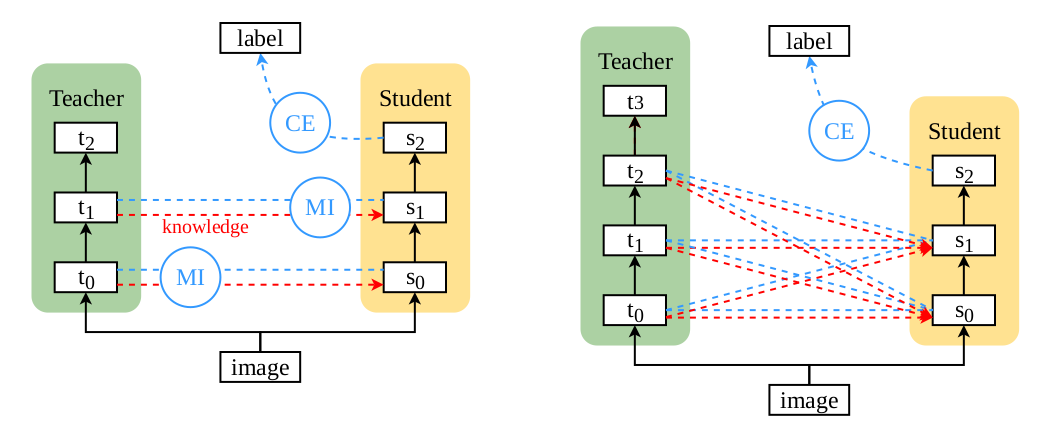
\includegraphics[width=0.9\textwidth]{method_scheme.png}
    \caption{Схема метода дистилляции Sungsoo Ahn (слева) и предлагаемого нами метода (справа)}
    \label{fig:method_scheme}
\end{figure}

Схема нашего метода, в сравнении с уже упомянутым методом Sungsoo Ahn\cite{Ahn_2019_CVPR}, изображена на рисунке \ref{fig:method_scheme}.


\subsection{Вариационная максимизация информации}

Функция потерь должна быть минимизирована относительно параметров модели ученика. Однако, сделать это будет сложно, так как трудно вычислить взаимную информацию.

Вместо этого используется вариационная нижняя граница для каждого члена взаимной информации $I(\bold{t}; \bold{s})$,
в которой определяется вариационное распределение $q(\bold{t}|\bold{s})$, которое аппроксимирует $p(\bold{t}|\bold{s})$:

\begin{multline}
    I(\bold{t}; \bold{s}) = H(\bold{t}) - H(\bold{t} | \bold{s}) =  H(\bold{t}) + \mathbb{E}_{\bold{t},\bold{s}}[\log{p(\bold{t}|\bold{s})}] \\
    + H(\bold{t}) + \mathbb{E}_{\bold{t},\bold{s}}[\log{q(\bold{t}|\bold{s})}] + \mathbb{E}_{\bold{s}}[D_{\text{KL}}(p(\bold{t}|\bold{s})||q(\bold{t}|\bold{s}))] \\
    \geq H(\bold{t}) + \mathbb{E}_{\bold{t},\bold{s}}[\log{q(\bold{t}|\bold{s})}].
\end{multline}

Данная техника известна как вариационная максимизация информации \cite{barber2004algorithm}. Применяя её к каждому члену взаимной информации в функции потерь, получим:

$$ \mathcal{L} = \beta \mathcal{L}_\text{CE} - (1 - \beta){\sum_{i=1}^T \sum_{j=1}^S \lambda_{i, j} \mathbb{E}_{\bold{t},\bold{s}}[\log{q(\bold{t}^{(i)}|\bold{s}^{(j)})}] }.$$

Эта новая функция потерь минимизируется относительно параметров модели ученика и вариационного распределения $q(\bold{t}|\bold{s})$.
Стоит обратить внимание, что энтропия $H(\bold{t})$ убрана из выражения, так как не зависит от оптимизируемых параметров.
Также второй член в функции потерь можно интерпретировать как максимизацию условной вероятности
соответствия активациям выбранных слоев из модели учителя.
Таким образом, сеть учеников получает сжатые знания, необходимые для восстановления активаций выбранных слоев в модели учителя.

Мы выбираем вариационное распределение $q(\bold{t}|\bold{s})$, как нормальное распределение с средним $\bmu(\cdot)$ и
стандратным отклонением $\bsigma$. При этом,  $\bmu(\cdot)$ является функцией от $\bold{s}$, а $\bsigma$ - нет.
Параметризация  $\bmu(\cdot)$ и $\bsigma$ зависит от типа слоя, которому соответствует $\bold{t}$,
и в процессе дистилляции эти параметры оптимизируются вместе с параметрами модели ученика.

Если $\bold{t}$ соответствует свёрточному слою сети учителя с размерностями активаций, обозначающими канал, высоту и ширину соответственно,
то есть $\bold{t} \in \mathbb{R}^{С \times H \times W}$, вариационное распределение имеет вид:

\begin{multline}
    -\log{q(\bold{t}|\bold{s})} = -\sum_{c=1}^{C}  \sum_{h=1}^{H} \sum_{w=1}^{W} \log{q(t_{c,h,w}|\bold{s})} = \\
    = \sum_{c=1}^{C}  \sum_{h=1}^{H} \sum_{w=1}^{W} \log{\sigma_c} + \frac{(t_{c,h,w} - \mu_{c,h,w}(\bold{s}))^2}{2\sigma_c^2} + constant.
\end{multline}

Рассмотрим все обозначения в данном выражении. Под $t_{c,h,w}$ обозначается скалярный компонент $\bold{t}$, взятый по индексу $(c, h, w)$.
Кроме того, $\bmu(\bold{s})$ представляет собой нейронную сеть из нескольких свёрточных слоёв, на вход которой подаются активации $\bold{s}$ слоя ученика,
а выход имеет размерность, совпадающую с размерностью  $\bold{t}$ слоя учителя. Стандартное отклонение задаём таким образом,
чтобы оно было положительное, в нашем случае:
$$\sigma^2_c = \log{(1 + e^{\alpha_c})} + \epsilon,$$
где $\alpha_c \in \mathbb{R} $ - обучаемый параметр и $\epsilon$ --- минимальное значение отклонения, заданное для численной устойчивости.

Если $\bold{t}$ соответствует линейному слою сети учителя с размерностью $N$, то есть $\bold{t} \in \mathbb{R}^{N}$,
тогда вариационное распределение имеет вид:

\begin{multline}
    -\log{q(\bold{t}|\bold{s})} = -\sum_{n=1}^{N}  \log{q(t_{n}|\bold{s})} = \\
    = \sum_{n=1}^{N} \log{\sigma_n} + \frac{(t_n - \mu_n(\bold{s}))^2}{2\sigma_n^2} + constant.
\end{multline}

В данном выражении обозначения $t_{n}$ и $\sigma_n$ аналогичны тем, что представлены выше, а $\bmu(\bold{s})$ представляет собой линейную модель,
так же отображающую активации после слоя $\bold{s}$ студента в вектор размерности $N$.

